\begin{figure}[htbp]
    \centering
    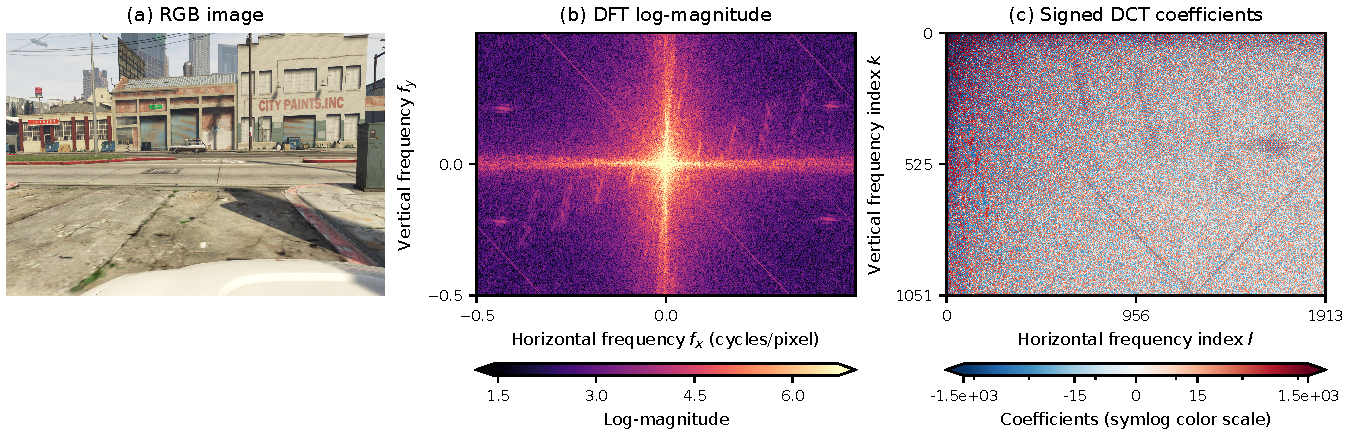
\includegraphics[width=\textwidth]{figures/frequency_representations_00003_theory.pdf}
    \caption[Global DFT and DCT representations]{%
    \textbf{Global frequency-domain representations of a GTA5 image.} (a) RGB input; (b) channel-averaged DFT magnitudes, computed via FFT and displayed after centering and $\log(1+x)$ scaling; (c) signed, channel-averaged unnormalized DCT-II coefficients. Both transforms are applied globally and independently to each RGB channel. Zero frequency is located at the center of (b) and the upper-left corner of (c). The maps are shown before the spatial standardization used for model input. Panel (c) uses a symmetric logarithmic color scale for visualization only. For visibility, the color limits in (b) are the 0.5th and 99.5th percentiles; in (c), they are symmetric around zero, using the 99.5th percentile of absolute values. The two color scales are independent. Source: own illustration based on an image from GTA5~\cite{gta5}.}
    \label{fig:frequency_representations_00003_theory}
\end{figure}
